% Options for packages loaded elsewhere
\PassOptionsToPackage{unicode}{hyperref}
\PassOptionsToPackage{hyphens}{url}
\PassOptionsToPackage{dvipsnames,svgnames,x11names}{xcolor}
%
\documentclass[
  letterpaper,
  DIV=11,
  numbers=noendperiod]{scrartcl}

\usepackage{amsmath,amssymb}
\usepackage{iftex}
\ifPDFTeX
  \usepackage[T1]{fontenc}
  \usepackage[utf8]{inputenc}
  \usepackage{textcomp} % provide euro and other symbols
\else % if luatex or xetex
  \usepackage{unicode-math}
  \defaultfontfeatures{Scale=MatchLowercase}
  \defaultfontfeatures[\rmfamily]{Ligatures=TeX,Scale=1}
\fi
\usepackage{lmodern}
\ifPDFTeX\else  
    % xetex/luatex font selection
\fi
% Use upquote if available, for straight quotes in verbatim environments
\IfFileExists{upquote.sty}{\usepackage{upquote}}{}
\IfFileExists{microtype.sty}{% use microtype if available
  \usepackage[]{microtype}
  \UseMicrotypeSet[protrusion]{basicmath} % disable protrusion for tt fonts
}{}
\makeatletter
\@ifundefined{KOMAClassName}{% if non-KOMA class
  \IfFileExists{parskip.sty}{%
    \usepackage{parskip}
  }{% else
    \setlength{\parindent}{0pt}
    \setlength{\parskip}{6pt plus 2pt minus 1pt}}
}{% if KOMA class
  \KOMAoptions{parskip=half}}
\makeatother
\usepackage{xcolor}
\setlength{\emergencystretch}{3em} % prevent overfull lines
\setcounter{secnumdepth}{-\maxdimen} % remove section numbering
% Make \paragraph and \subparagraph free-standing
\makeatletter
\ifx\paragraph\undefined\else
  \let\oldparagraph\paragraph
  \renewcommand{\paragraph}{
    \@ifstar
      \xxxParagraphStar
      \xxxParagraphNoStar
  }
  \newcommand{\xxxParagraphStar}[1]{\oldparagraph*{#1}\mbox{}}
  \newcommand{\xxxParagraphNoStar}[1]{\oldparagraph{#1}\mbox{}}
\fi
\ifx\subparagraph\undefined\else
  \let\oldsubparagraph\subparagraph
  \renewcommand{\subparagraph}{
    \@ifstar
      \xxxSubParagraphStar
      \xxxSubParagraphNoStar
  }
  \newcommand{\xxxSubParagraphStar}[1]{\oldsubparagraph*{#1}\mbox{}}
  \newcommand{\xxxSubParagraphNoStar}[1]{\oldsubparagraph{#1}\mbox{}}
\fi
\makeatother

\usepackage{color}
\usepackage{fancyvrb}
\newcommand{\VerbBar}{|}
\newcommand{\VERB}{\Verb[commandchars=\\\{\}]}
\DefineVerbatimEnvironment{Highlighting}{Verbatim}{commandchars=\\\{\}}
% Add ',fontsize=\small' for more characters per line
\usepackage{framed}
\definecolor{shadecolor}{RGB}{241,243,245}
\newenvironment{Shaded}{\begin{snugshade}}{\end{snugshade}}
\newcommand{\AlertTok}[1]{\textcolor[rgb]{0.68,0.00,0.00}{#1}}
\newcommand{\AnnotationTok}[1]{\textcolor[rgb]{0.37,0.37,0.37}{#1}}
\newcommand{\AttributeTok}[1]{\textcolor[rgb]{0.40,0.45,0.13}{#1}}
\newcommand{\BaseNTok}[1]{\textcolor[rgb]{0.68,0.00,0.00}{#1}}
\newcommand{\BuiltInTok}[1]{\textcolor[rgb]{0.00,0.23,0.31}{#1}}
\newcommand{\CharTok}[1]{\textcolor[rgb]{0.13,0.47,0.30}{#1}}
\newcommand{\CommentTok}[1]{\textcolor[rgb]{0.37,0.37,0.37}{#1}}
\newcommand{\CommentVarTok}[1]{\textcolor[rgb]{0.37,0.37,0.37}{\textit{#1}}}
\newcommand{\ConstantTok}[1]{\textcolor[rgb]{0.56,0.35,0.01}{#1}}
\newcommand{\ControlFlowTok}[1]{\textcolor[rgb]{0.00,0.23,0.31}{\textbf{#1}}}
\newcommand{\DataTypeTok}[1]{\textcolor[rgb]{0.68,0.00,0.00}{#1}}
\newcommand{\DecValTok}[1]{\textcolor[rgb]{0.68,0.00,0.00}{#1}}
\newcommand{\DocumentationTok}[1]{\textcolor[rgb]{0.37,0.37,0.37}{\textit{#1}}}
\newcommand{\ErrorTok}[1]{\textcolor[rgb]{0.68,0.00,0.00}{#1}}
\newcommand{\ExtensionTok}[1]{\textcolor[rgb]{0.00,0.23,0.31}{#1}}
\newcommand{\FloatTok}[1]{\textcolor[rgb]{0.68,0.00,0.00}{#1}}
\newcommand{\FunctionTok}[1]{\textcolor[rgb]{0.28,0.35,0.67}{#1}}
\newcommand{\ImportTok}[1]{\textcolor[rgb]{0.00,0.46,0.62}{#1}}
\newcommand{\InformationTok}[1]{\textcolor[rgb]{0.37,0.37,0.37}{#1}}
\newcommand{\KeywordTok}[1]{\textcolor[rgb]{0.00,0.23,0.31}{\textbf{#1}}}
\newcommand{\NormalTok}[1]{\textcolor[rgb]{0.00,0.23,0.31}{#1}}
\newcommand{\OperatorTok}[1]{\textcolor[rgb]{0.37,0.37,0.37}{#1}}
\newcommand{\OtherTok}[1]{\textcolor[rgb]{0.00,0.23,0.31}{#1}}
\newcommand{\PreprocessorTok}[1]{\textcolor[rgb]{0.68,0.00,0.00}{#1}}
\newcommand{\RegionMarkerTok}[1]{\textcolor[rgb]{0.00,0.23,0.31}{#1}}
\newcommand{\SpecialCharTok}[1]{\textcolor[rgb]{0.37,0.37,0.37}{#1}}
\newcommand{\SpecialStringTok}[1]{\textcolor[rgb]{0.13,0.47,0.30}{#1}}
\newcommand{\StringTok}[1]{\textcolor[rgb]{0.13,0.47,0.30}{#1}}
\newcommand{\VariableTok}[1]{\textcolor[rgb]{0.07,0.07,0.07}{#1}}
\newcommand{\VerbatimStringTok}[1]{\textcolor[rgb]{0.13,0.47,0.30}{#1}}
\newcommand{\WarningTok}[1]{\textcolor[rgb]{0.37,0.37,0.37}{\textit{#1}}}

\providecommand{\tightlist}{%
  \setlength{\itemsep}{0pt}\setlength{\parskip}{0pt}}\usepackage{longtable,booktabs,array}
\usepackage{calc} % for calculating minipage widths
% Correct order of tables after \paragraph or \subparagraph
\usepackage{etoolbox}
\makeatletter
\patchcmd\longtable{\par}{\if@noskipsec\mbox{}\fi\par}{}{}
\makeatother
% Allow footnotes in longtable head/foot
\IfFileExists{footnotehyper.sty}{\usepackage{footnotehyper}}{\usepackage{footnote}}
\makesavenoteenv{longtable}
\usepackage{graphicx}
\makeatletter
\def\maxwidth{\ifdim\Gin@nat@width>\linewidth\linewidth\else\Gin@nat@width\fi}
\def\maxheight{\ifdim\Gin@nat@height>\textheight\textheight\else\Gin@nat@height\fi}
\makeatother
% Scale images if necessary, so that they will not overflow the page
% margins by default, and it is still possible to overwrite the defaults
% using explicit options in \includegraphics[width, height, ...]{}
\setkeys{Gin}{width=\maxwidth,height=\maxheight,keepaspectratio}
% Set default figure placement to htbp
\makeatletter
\def\fps@figure{htbp}
\makeatother

\KOMAoption{captions}{tableheading}
\makeatletter
\@ifpackageloaded{caption}{}{\usepackage{caption}}
\AtBeginDocument{%
\ifdefined\contentsname
  \renewcommand*\contentsname{Tabla de contenidos}
\else
  \newcommand\contentsname{Tabla de contenidos}
\fi
\ifdefined\listfigurename
  \renewcommand*\listfigurename{Listado de Figuras}
\else
  \newcommand\listfigurename{Listado de Figuras}
\fi
\ifdefined\listtablename
  \renewcommand*\listtablename{Listado de Tablas}
\else
  \newcommand\listtablename{Listado de Tablas}
\fi
\ifdefined\figurename
  \renewcommand*\figurename{Figura}
\else
  \newcommand\figurename{Figura}
\fi
\ifdefined\tablename
  \renewcommand*\tablename{Tabla}
\else
  \newcommand\tablename{Tabla}
\fi
}
\@ifpackageloaded{float}{}{\usepackage{float}}
\floatstyle{ruled}
\@ifundefined{c@chapter}{\newfloat{codelisting}{h}{lop}}{\newfloat{codelisting}{h}{lop}[chapter]}
\floatname{codelisting}{Listado}
\newcommand*\listoflistings{\listof{codelisting}{Listado de Listados}}
\makeatother
\makeatletter
\makeatother
\makeatletter
\@ifpackageloaded{caption}{}{\usepackage{caption}}
\@ifpackageloaded{subcaption}{}{\usepackage{subcaption}}
\makeatother

\ifLuaTeX
\usepackage[bidi=basic]{babel}
\else
\usepackage[bidi=default]{babel}
\fi
\babelprovide[main,import]{spanish}
% get rid of language-specific shorthands (see #6817):
\let\LanguageShortHands\languageshorthands
\def\languageshorthands#1{}
\ifLuaTeX
  \usepackage{selnolig}  % disable illegal ligatures
\fi
\usepackage{bookmark}

\IfFileExists{xurl.sty}{\usepackage{xurl}}{} % add URL line breaks if available
\urlstyle{same} % disable monospaced font for URLs
\hypersetup{
  pdftitle={Tarea 8},
  pdfauthor={MARIA BELEN RAURA ANTE},
  pdflang={es},
  colorlinks=true,
  linkcolor={blue},
  filecolor={Maroon},
  citecolor={Blue},
  urlcolor={Blue},
  pdfcreator={LaTeX via pandoc}}


\title{Tarea 8}
\author{MARIA BELEN RAURA ANTE}
\date{}

\begin{document}
\maketitle

\renewcommand*\contentsname{Tabla de Contenidos}
{
\hypersetup{linkcolor=}
\setcounter{tocdepth}{3}
\tableofcontents
}

\section{CONJUNTO DE EJERCICIOS}\label{conjunto-de-ejercicios}

\begin{enumerate}
\def\labelenumi{\arabic{enumi}.}
\tightlist
\item
  Dados los datos:
\end{enumerate}

\begin{longtable}[]{@{}
  >{\raggedright\arraybackslash}p{(\columnwidth - 20\tabcolsep) * \real{0.0667}}
  >{\raggedright\arraybackslash}p{(\columnwidth - 20\tabcolsep) * \real{0.0933}}
  >{\raggedright\arraybackslash}p{(\columnwidth - 20\tabcolsep) * \real{0.0933}}
  >{\raggedright\arraybackslash}p{(\columnwidth - 20\tabcolsep) * \real{0.0933}}
  >{\raggedright\arraybackslash}p{(\columnwidth - 20\tabcolsep) * \real{0.0933}}
  >{\raggedright\arraybackslash}p{(\columnwidth - 20\tabcolsep) * \real{0.0933}}
  >{\raggedright\arraybackslash}p{(\columnwidth - 20\tabcolsep) * \real{0.0933}}
  >{\raggedright\arraybackslash}p{(\columnwidth - 20\tabcolsep) * \real{0.0933}}
  >{\raggedright\arraybackslash}p{(\columnwidth - 20\tabcolsep) * \real{0.0933}}
  >{\raggedright\arraybackslash}p{(\columnwidth - 20\tabcolsep) * \real{0.0933}}
  >{\raggedright\arraybackslash}p{(\columnwidth - 20\tabcolsep) * \real{0.0933}}@{}}
\toprule\noalign{}
\begin{minipage}[b]{\linewidth}\raggedright
xi
\end{minipage} & \begin{minipage}[b]{\linewidth}\raggedright
4.0
\end{minipage} & \begin{minipage}[b]{\linewidth}\raggedright
4.2
\end{minipage} & \begin{minipage}[b]{\linewidth}\raggedright
4.5
\end{minipage} & \begin{minipage}[b]{\linewidth}\raggedright
4.7
\end{minipage} & \begin{minipage}[b]{\linewidth}\raggedright
5.1
\end{minipage} & \begin{minipage}[b]{\linewidth}\raggedright
5.5
\end{minipage} & \begin{minipage}[b]{\linewidth}\raggedright
5.9
\end{minipage} & \begin{minipage}[b]{\linewidth}\raggedright
6.3
\end{minipage} & \begin{minipage}[b]{\linewidth}\raggedright
6.8
\end{minipage} & \begin{minipage}[b]{\linewidth}\raggedright
7.1
\end{minipage} \\
\midrule\noalign{}
\endhead
\bottomrule\noalign{}
\endlastfoot
yi & 102.56 & 130.11 & 113.18 & 142.05 & 167.53 & 195.14 & 224.87 &
256.73 & 299.50 & 326.72 \\
\end{longtable}

\begin{enumerate}
\def\labelenumi{\alph{enumi}.}
\item
  Construya el polinomio por mínimos cuadrados de grado 1 y calcule el
  error.
\item
  Construya el polinomio por mínimos cuadrados de grado 2 y calcule el
  error.
\item
  Construya el polinomio por mínimos cuadrados de grado 3 y calcule el
  error.
\item
  Construya el polinomio por mínimos cuadrados de la forma (
  be\^{}\{ax\} ) y calcule el error.
\item
  Construya el polinomio por mínimos cuadrados de la forma ( bx\^{}a ) y
  calcule el error.
\end{enumerate}

\section{Módulo utilizado para la función
resultante}\label{muxf3dulo-utilizado-para-la-funciuxf3n-resultante}

Dentro de la librería Scipy existe una función en optimize que nos
permite minimizar el error al cuadrado de la distancia entre la imagen
de una función aproximada y una serie de pares ordenados. Realmente, se
usa un sistema de ecuaciones para consagrar los parámetros finales de la
función resultante. La parte del error se pensó obteniendo un promedio
de todos los errores relativos con ayuda de numpy, aprovechando que está
importada. Esta es la pieza de código que graficará los resultados y
calculará el error:

\begin{Shaded}
\begin{Highlighting}[]

\ImportTok{import}\NormalTok{ sympy }\ImportTok{as}\NormalTok{ sym}
\ImportTok{import}\NormalTok{ numpy }\ImportTok{as}\NormalTok{ np}
\ImportTok{import}\NormalTok{ matplotlib.pyplot }\ImportTok{as}\NormalTok{ plt}
\ImportTok{from}\NormalTok{ scipy.optimize }\ImportTok{import}\NormalTok{ curve\_fit}

\KeywordTok{def}\NormalTok{ leasts\_squares\_graphic(func, x\_real\_points, y\_real\_points):}
\NormalTok{    x\_plot }\OperatorTok{=}\NormalTok{ np.linspace(}\BuiltInTok{min}\NormalTok{(x\_real\_points), }\BuiltInTok{max}\NormalTok{(x\_real\_points), }\DecValTok{100}\NormalTok{)}
\NormalTok{    y\_plot }\OperatorTok{=}\NormalTok{ func(x\_plot)}
    
    \CommentTok{\# Graficar los datos originales y la curva ajustada}
\NormalTok{    plt.scatter(x\_real\_points, y\_real\_points, label}\OperatorTok{=}\StringTok{\textquotesingle{}Datos\textquotesingle{}}\NormalTok{, color}\OperatorTok{=}\StringTok{\textquotesingle{}red\textquotesingle{}}\NormalTok{)}
\NormalTok{    plt.plot(x\_plot, y\_plot, label}\OperatorTok{=}\StringTok{\textquotesingle{}Ajuste de la función final\textquotesingle{}}\NormalTok{, color}\OperatorTok{=}\StringTok{\textquotesingle{}blue\textquotesingle{}}\NormalTok{)}
\NormalTok{    plt.xlabel(}\StringTok{\textquotesingle{}x\textquotesingle{}}\NormalTok{)}
\NormalTok{    plt.ylabel(}\StringTok{\textquotesingle{}y\textquotesingle{}}\NormalTok{)}
\NormalTok{    plt.legend()}
\NormalTok{    plt.show()}

\KeywordTok{def}\NormalTok{ calculate\_error(func, x\_real\_points, y\_real\_points):}
\NormalTok{    x\_real\_points }\OperatorTok{=}\NormalTok{ np.array(x\_real\_points)}
\NormalTok{    y\_approx\_points }\OperatorTok{=}\NormalTok{ func(x\_real\_points)}
\NormalTok{    error }\OperatorTok{=} \BuiltInTok{abs}\NormalTok{(x\_real\_points }\OperatorTok{{-}}\NormalTok{ y\_approx\_points)}
\NormalTok{    r\_error }\OperatorTok{=}\NormalTok{ np.}\BuiltInTok{sum}\NormalTok{(error }\OperatorTok{/}\NormalTok{ y\_real\_points) }\OperatorTok{/} \BuiltInTok{len}\NormalTok{(y\_real\_points)}
    
    \ControlFlowTok{return}\NormalTok{ r\_error}
    
\end{Highlighting}
\end{Shaded}

\section{Conjunto de ejercicios}\label{conjunto-de-ejercicios-1}

\subsection{Ejercicio 1}\label{ejercicio-1}

Dados los datos:

\begin{Shaded}
\begin{Highlighting}[]
\NormalTok{x\_ej1 }\OperatorTok{=}\NormalTok{ [}\DecValTok{4}\NormalTok{, }\FloatTok{4.2}\NormalTok{, }\FloatTok{4.5}\NormalTok{, }\FloatTok{4.7}\NormalTok{, }\FloatTok{5.1}\NormalTok{, }\FloatTok{5.5}\NormalTok{, }\FloatTok{5.9}\NormalTok{, }\FloatTok{6.3}\NormalTok{, }\FloatTok{6.8}\NormalTok{, }\FloatTok{7.1}\NormalTok{]}
\NormalTok{y\_ej1 }\OperatorTok{=}\NormalTok{ [}\FloatTok{102.56}\NormalTok{, }\FloatTok{130.11}\NormalTok{, }\FloatTok{113.18}\NormalTok{, }\FloatTok{142.05}\NormalTok{, }\FloatTok{167.53}\NormalTok{, }\FloatTok{195.14}\NormalTok{, }\FloatTok{224.87}\NormalTok{, }\FloatTok{256.73}\NormalTok{, }\FloatTok{299.50}\NormalTok{, }\FloatTok{326.72}\NormalTok{]}
\end{Highlighting}
\end{Shaded}

\subsubsection{Literal a)}\label{literal-a}

Construya el polinomio por mínimos cuadrados de grado 1 y calcule el
error.

\begin{Shaded}
\begin{Highlighting}[]

\KeywordTok{def}\NormalTok{ func(x, a, b):}
    \ControlFlowTok{return}\NormalTok{ a}\OperatorTok{*}\NormalTok{x }\OperatorTok{+}\NormalTok{ b}

\CommentTok{\# Minimizando el error}
\NormalTok{popt, pcov }\OperatorTok{=}\NormalTok{ curve\_fit(func, x\_ej1, y\_ej1)}
\NormalTok{a, b }\OperatorTok{=}\NormalTok{ popt}

\CommentTok{\# Imprimiendo la función resultante y el error}
\NormalTok{x\_sym }\OperatorTok{=}\NormalTok{ sym.symbols(}\StringTok{"x"}\NormalTok{)}
\NormalTok{func\_sym }\OperatorTok{=} \BuiltInTok{round}\NormalTok{(a, }\DecValTok{2}\NormalTok{)}\OperatorTok{*}\NormalTok{x\_sym }\OperatorTok{+} \BuiltInTok{round}\NormalTok{(b, }\DecValTok{2}\NormalTok{)}
\BuiltInTok{print}\NormalTok{(}\SpecialStringTok{f"La función resultante es: }\SpecialCharTok{\{}\NormalTok{func\_sym}\SpecialCharTok{\}}\SpecialStringTok{"}\NormalTok{)}

\NormalTok{r\_error }\OperatorTok{=}\NormalTok{ calculate\_error(}\KeywordTok{lambda}\NormalTok{ x: a}\OperatorTok{*}\NormalTok{x }\OperatorTok{+}\NormalTok{ b, x\_ej1, y\_ej1)}
\BuiltInTok{print}\NormalTok{(}\SpecialStringTok{f"El error relativo en todos los puntos promedio es: }\SpecialCharTok{\{}\NormalTok{r\_error}\SpecialCharTok{\}}\SpecialStringTok{"}\NormalTok{)}

\CommentTok{\# Graficando}
\NormalTok{leasts\_squares\_graphic(}\KeywordTok{lambda}\NormalTok{ x: a}\OperatorTok{*}\NormalTok{x }\OperatorTok{+}\NormalTok{ b, x\_ej1, y\_ej1)}
\end{Highlighting}
\end{Shaded}

\begin{verbatim}
La función resultante es: 71.61*x - 191.57
El error relativo en todos los puntos promedio es: 0.9708703736157682
\end{verbatim}

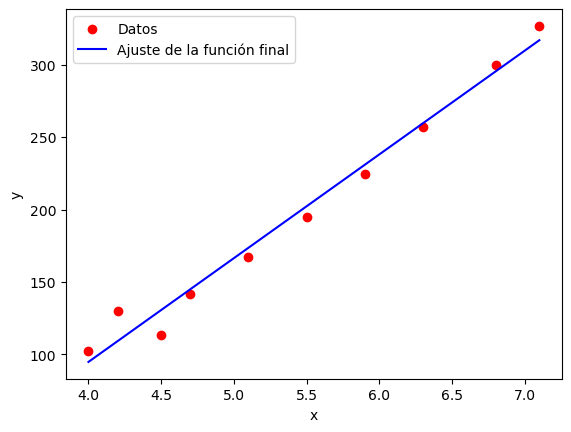
\includegraphics{Tarea8_MN_files/figure-pdf/cell-4-output-2.png}

Definimos primero la función lineal que se ajustará minimamente a los
puntos dados. Para este y los siguientes casos, ``popt'' contiene las
variables ``a'' o ``b'' que modifican a la función inicial linear.

\subsubsection{Literal b)}\label{literal-b}

Construya el polinomio por mínimos cuadrados de grado 2 y calcule el
error.

Solamente modificaremos la función que será un parámetro por una
cuadrática con 3 incógnitas (a, b, c).

\begin{Shaded}
\begin{Highlighting}[]

\KeywordTok{def}\NormalTok{ func(x, a, b, c):}
    \ControlFlowTok{return}\NormalTok{ a}\OperatorTok{*}\NormalTok{x}\OperatorTok{**}\DecValTok{2} \OperatorTok{+}\NormalTok{ b}\OperatorTok{*}\NormalTok{x }\OperatorTok{+}\NormalTok{ c}

\CommentTok{\# Minimizando el error}
\NormalTok{popt, pcov }\OperatorTok{=}\NormalTok{ curve\_fit(func, x\_ej1, y\_ej1)}
\NormalTok{a, b, c }\OperatorTok{=}\NormalTok{ popt}

\CommentTok{\# Imprimiendo la función resultante y el error}
\NormalTok{x\_sym }\OperatorTok{=}\NormalTok{ sym.symbols(}\StringTok{"x"}\NormalTok{)}
\NormalTok{func\_sym }\OperatorTok{=} \BuiltInTok{round}\NormalTok{(a, }\DecValTok{2}\NormalTok{)}\OperatorTok{*}\NormalTok{x\_sym}\OperatorTok{**}\DecValTok{2} \OperatorTok{+} \BuiltInTok{round}\NormalTok{(b, }\DecValTok{2}\NormalTok{)}\OperatorTok{*}\NormalTok{x\_sym }\OperatorTok{+} \BuiltInTok{round}\NormalTok{(c, }\DecValTok{2}\NormalTok{)}
\BuiltInTok{print}\NormalTok{(}\SpecialStringTok{f"La función resultante es: }\SpecialCharTok{\{}\NormalTok{func\_sym}\SpecialCharTok{\}}\SpecialStringTok{"}\NormalTok{)}

\NormalTok{r\_error }\OperatorTok{=}\NormalTok{ calculate\_error(}\KeywordTok{lambda}\NormalTok{ x: a}\OperatorTok{*}\NormalTok{x}\OperatorTok{**}\DecValTok{2} \OperatorTok{+}\NormalTok{ b}\OperatorTok{*}\NormalTok{x }\OperatorTok{+}\NormalTok{ c, x\_ej1, y\_ej1)}
\BuiltInTok{print}\NormalTok{(}\SpecialStringTok{f"El error relativo en todos los puntos promedio es: }\SpecialCharTok{\{}\NormalTok{r\_error}\SpecialCharTok{\}}\SpecialStringTok{"}\NormalTok{)}

\CommentTok{\# Graficando}
\NormalTok{leasts\_squares\_graphic(}\KeywordTok{lambda}\NormalTok{ x: a}\OperatorTok{*}\NormalTok{x}\OperatorTok{**}\DecValTok{2} \OperatorTok{+}\NormalTok{ b}\OperatorTok{*}\NormalTok{x }\OperatorTok{+}\NormalTok{ c, x\_ej1, y\_ej1)}
\end{Highlighting}
\end{Shaded}

\begin{verbatim}
La función resultante es: 8.22*x**2 - 19.31*x + 51.0
El error relativo en todos los puntos promedio es: 0.9737540796582553
\end{verbatim}

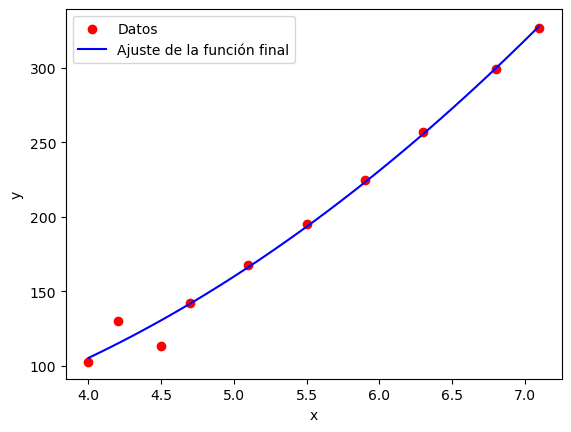
\includegraphics{Tarea8_MN_files/figure-pdf/cell-5-output-2.png}

\subsubsection{Literal c)}\label{literal-c}

Construya el polinomio por mínimos cuadrados de grado 3 y calcule el
error.

\begin{Shaded}
\begin{Highlighting}[]

\KeywordTok{def}\NormalTok{ func(x, a, b, c, d):}
    \ControlFlowTok{return}\NormalTok{ a}\OperatorTok{*}\NormalTok{x}\OperatorTok{**}\DecValTok{3} \OperatorTok{+}\NormalTok{ b}\OperatorTok{*}\NormalTok{x}\OperatorTok{**}\DecValTok{2} \OperatorTok{+}\NormalTok{ c}\OperatorTok{*}\NormalTok{x }\OperatorTok{+}\NormalTok{ d}

\CommentTok{\# Minimizando el error}
\NormalTok{popt, pcov }\OperatorTok{=}\NormalTok{ curve\_fit(func, x\_ej1, y\_ej1)}
\NormalTok{a, b, c, d }\OperatorTok{=}\NormalTok{ popt}

\CommentTok{\# Imprimiendo la función resultante y el error}
\NormalTok{x\_sym }\OperatorTok{=}\NormalTok{ sym.symbols(}\StringTok{"x"}\NormalTok{)}
\NormalTok{func\_sym }\OperatorTok{=} \BuiltInTok{round}\NormalTok{(a, }\DecValTok{2}\NormalTok{)}\OperatorTok{*}\NormalTok{x\_sym}\OperatorTok{**}\DecValTok{3} \OperatorTok{+} \BuiltInTok{round}\NormalTok{(b, }\DecValTok{2}\NormalTok{)}\OperatorTok{*}\NormalTok{x\_sym}\OperatorTok{**}\DecValTok{2} \OperatorTok{+} \BuiltInTok{round}\NormalTok{(c, }\DecValTok{2}\NormalTok{)}\OperatorTok{*}\NormalTok{x\_sym }\OperatorTok{+} \BuiltInTok{round}\NormalTok{(d, }\DecValTok{2}\NormalTok{)}
\BuiltInTok{print}\NormalTok{(}\SpecialStringTok{f"La función resultante es: }\SpecialCharTok{\{}\NormalTok{func\_sym}\SpecialCharTok{\}}\SpecialStringTok{"}\NormalTok{)}

\NormalTok{r\_error }\OperatorTok{=}\NormalTok{ calculate\_error(}\KeywordTok{lambda}\NormalTok{ x: a}\OperatorTok{*}\NormalTok{x}\OperatorTok{**}\DecValTok{3} \OperatorTok{+}\NormalTok{ b}\OperatorTok{*}\NormalTok{x}\OperatorTok{**}\DecValTok{2} \OperatorTok{+}\NormalTok{ c}\OperatorTok{*}\NormalTok{x }\OperatorTok{+}\NormalTok{ d, x\_ej1, y\_ej1)}
\BuiltInTok{print}\NormalTok{(}\SpecialStringTok{f"El error relativo en todos los puntos promedio es: }\SpecialCharTok{\{}\NormalTok{r\_error}\SpecialCharTok{\}}\SpecialStringTok{"}\NormalTok{)}

\CommentTok{\# Graficando}
\NormalTok{leasts\_squares\_graphic(}\KeywordTok{lambda}\NormalTok{ x: a}\OperatorTok{*}\NormalTok{x}\OperatorTok{**}\DecValTok{3} \OperatorTok{+}\NormalTok{ b}\OperatorTok{*}\NormalTok{x}\OperatorTok{**}\DecValTok{2} \OperatorTok{+}\NormalTok{ c}\OperatorTok{*}\NormalTok{x }\OperatorTok{+}\NormalTok{ d, x\_ej1, y\_ej1)}
\end{Highlighting}
\end{Shaded}

\begin{verbatim}
La función resultante es: -2.61*x**3 + 51.56*x**2 - 254.88*x + 469.16
El error relativo en todos los puntos promedio es: 0.9737126806863465
\end{verbatim}

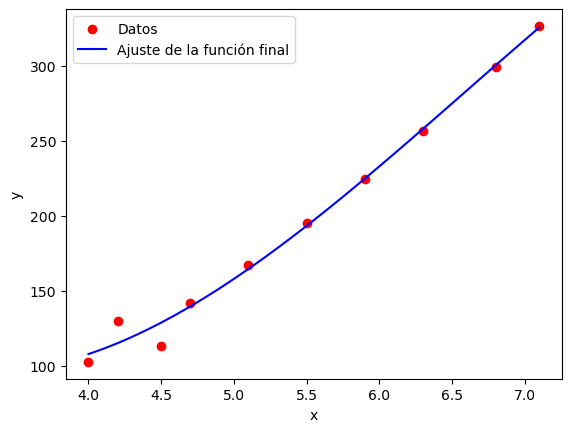
\includegraphics{Tarea8_MN_files/figure-pdf/cell-6-output-2.png}

\subsubsection{Literal d)}\label{literal-d}

Construya el polinomio por mínimos cuadrados de la forma \(be^{ax}\) y
calcule el error.

\begin{Shaded}
\begin{Highlighting}[]

\KeywordTok{def}\NormalTok{ func(x, a, b):}
    \ControlFlowTok{return}\NormalTok{ b}\OperatorTok{*}\NormalTok{np.exp(a}\OperatorTok{*}\NormalTok{x)}

\CommentTok{\# Minimizando el error}
\NormalTok{popt, pcov }\OperatorTok{=}\NormalTok{ curve\_fit(func, x\_ej1, y\_ej1)}
\NormalTok{a, b }\OperatorTok{=}\NormalTok{ popt}

\CommentTok{\# Imprimiendo la función resultante y el error}
\NormalTok{x\_sym }\OperatorTok{=}\NormalTok{ sym.symbols(}\StringTok{"x"}\NormalTok{)}
\NormalTok{func\_sym }\OperatorTok{=} \BuiltInTok{round}\NormalTok{(b, }\DecValTok{2}\NormalTok{)}\OperatorTok{*}\NormalTok{sym.exp(}\BuiltInTok{round}\NormalTok{(a, }\DecValTok{2}\NormalTok{)}\OperatorTok{*}\NormalTok{x\_sym)}
\BuiltInTok{print}\NormalTok{(}\SpecialStringTok{f"La función resultante es: }\SpecialCharTok{\{}\NormalTok{func\_sym}\SpecialCharTok{\}}\SpecialStringTok{"}\NormalTok{)}

\NormalTok{r\_error }\OperatorTok{=}\NormalTok{ calculate\_error(}\KeywordTok{lambda}\NormalTok{ x: b}\OperatorTok{*}\NormalTok{np.exp(a}\OperatorTok{*}\NormalTok{x), x\_ej1, y\_ej1)}
\BuiltInTok{print}\NormalTok{(}\SpecialStringTok{f"El error relativo en todos los puntos promedio es: }\SpecialCharTok{\{}\NormalTok{r\_error}\SpecialCharTok{\}}\SpecialStringTok{"}\NormalTok{)}

\CommentTok{\# Graficando}
\NormalTok{leasts\_squares\_graphic(}\KeywordTok{lambda}\NormalTok{ x: b}\OperatorTok{*}\NormalTok{np.exp(a}\OperatorTok{*}\NormalTok{x), x\_ej1, y\_ej1)}
\end{Highlighting}
\end{Shaded}

\begin{verbatim}
La función resultante es: 26.84*exp(0.35*x)
El error relativo en todos los puntos promedio es: 0.979099530943642
\end{verbatim}

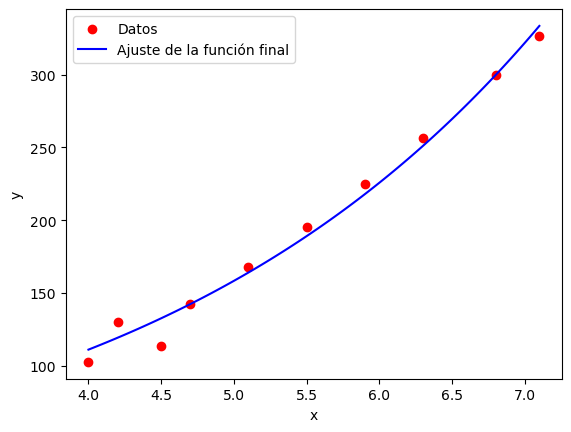
\includegraphics{Tarea8_MN_files/figure-pdf/cell-7-output-2.png}

\subsubsection{Literal e)}\label{literal-e}

Construya el polinomio por mínimos cuadrados de la forma \(bx^a\) y
calcule el error.

\begin{Shaded}
\begin{Highlighting}[]

\KeywordTok{def}\NormalTok{ func(x, a, b):}
    \ControlFlowTok{return}\NormalTok{ b}\OperatorTok{*}\NormalTok{x}\OperatorTok{**}\NormalTok{a}

\CommentTok{\# Minimizando el error}
\NormalTok{popt, pcov }\OperatorTok{=}\NormalTok{ curve\_fit(func, x\_ej1, y\_ej1)}
\NormalTok{a, b }\OperatorTok{=}\NormalTok{ popt}

\CommentTok{\# Imprimiendo la función resultante y el error}
\NormalTok{x\_sym }\OperatorTok{=}\NormalTok{ sym.symbols(}\StringTok{"x"}\NormalTok{)}
\NormalTok{func\_sym }\OperatorTok{=} \BuiltInTok{round}\NormalTok{(b, }\DecValTok{2}\NormalTok{)}\OperatorTok{*}\NormalTok{x\_sym}\OperatorTok{**}\BuiltInTok{round}\NormalTok{(a, }\DecValTok{2}\NormalTok{)}
\BuiltInTok{print}\NormalTok{(}\SpecialStringTok{f"La función resultante es: }\SpecialCharTok{\{}\NormalTok{func\_sym}\SpecialCharTok{\}}\SpecialStringTok{"}\NormalTok{)}

\NormalTok{r\_error }\OperatorTok{=}\NormalTok{ calculate\_error(}\KeywordTok{lambda}\NormalTok{ x: b}\OperatorTok{*}\NormalTok{x}\OperatorTok{**}\NormalTok{a, x\_ej1, y\_ej1)}
\BuiltInTok{print}\NormalTok{(}\SpecialStringTok{f"El error relativo en todos los puntos promedio es: }\SpecialCharTok{\{}\NormalTok{r\_error}\SpecialCharTok{\}}\SpecialStringTok{"}\NormalTok{)}

\CommentTok{\# Graficando}
\NormalTok{leasts\_squares\_graphic(}\KeywordTok{lambda}\NormalTok{ x: b}\OperatorTok{*}\NormalTok{x}\OperatorTok{**}\NormalTok{a, x\_ej1, y\_ej1)}
\end{Highlighting}
\end{Shaded}

\begin{verbatim}
La función resultante es: 6.28*x**2.02
El error relativo en todos los puntos promedio es: 0.9720570275812594
\end{verbatim}

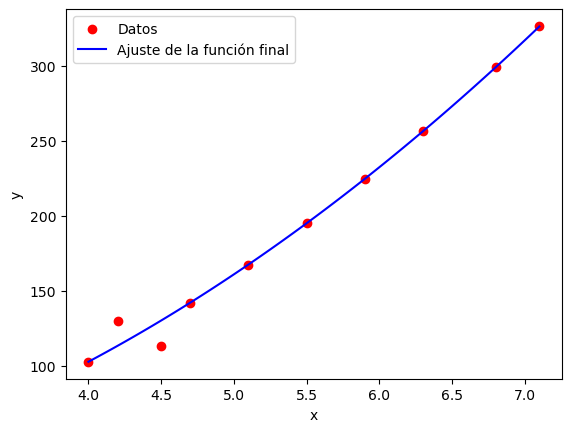
\includegraphics{Tarea8_MN_files/figure-pdf/cell-8-output-2.png}

\subsection{Ejercicio 2}\label{ejercicio-2}

Repita el ejercicio 5 para los siguientes datos.

\begin{Shaded}
\begin{Highlighting}[]
\NormalTok{x\_ej2 }\OperatorTok{=}\NormalTok{ [}\FloatTok{0.2}\NormalTok{, }\FloatTok{0.3}\NormalTok{, }\FloatTok{0.6}\NormalTok{, }\FloatTok{0.9}\NormalTok{, }\FloatTok{1.1}\NormalTok{, }\FloatTok{1.3}\NormalTok{, }\FloatTok{1.4}\NormalTok{, }\FloatTok{1.6}\NormalTok{]}
\NormalTok{y\_ej2 }\OperatorTok{=}\NormalTok{ [}\FloatTok{0.050446}\NormalTok{, }\FloatTok{0.098426}\NormalTok{, }\FloatTok{0.33277}\NormalTok{, }\FloatTok{0.72660}\NormalTok{, }\FloatTok{1.0972}\NormalTok{, }\FloatTok{1.5697}\NormalTok{, }\FloatTok{1.8487}\NormalTok{, }\FloatTok{2.5015}\NormalTok{]}
\end{Highlighting}
\end{Shaded}

\subsubsection{Literal a)}\label{literal-a-1}

Construya el polinomio por mínimos cuadrados de grado 1 y calcule el
error.

\begin{Shaded}
\begin{Highlighting}[]

\KeywordTok{def}\NormalTok{ func(x, a, b):}
    \ControlFlowTok{return}\NormalTok{ a}\OperatorTok{*}\NormalTok{x }\OperatorTok{+}\NormalTok{ b}

\CommentTok{\# Minimizando el error}
\NormalTok{popt, pcov }\OperatorTok{=}\NormalTok{ curve\_fit(func, x\_ej2, y\_ej2)}
\NormalTok{a, b }\OperatorTok{=}\NormalTok{ popt}

\CommentTok{\# Imprimiendo la función resultante y el error}
\NormalTok{x\_sym }\OperatorTok{=}\NormalTok{ sym.symbols(}\StringTok{"x"}\NormalTok{)}
\NormalTok{func\_sym }\OperatorTok{=} \BuiltInTok{round}\NormalTok{(a, }\DecValTok{2}\NormalTok{)}\OperatorTok{*}\NormalTok{x\_sym }\OperatorTok{+} \BuiltInTok{round}\NormalTok{(b, }\DecValTok{2}\NormalTok{)}
\BuiltInTok{print}\NormalTok{(}\SpecialStringTok{f"La función resultante es: }\SpecialCharTok{\{}\NormalTok{func\_sym}\SpecialCharTok{\}}\SpecialStringTok{"}\NormalTok{)}

\NormalTok{r\_error }\OperatorTok{=}\NormalTok{ calculate\_error(}\KeywordTok{lambda}\NormalTok{ x: a}\OperatorTok{*}\NormalTok{x }\OperatorTok{+}\NormalTok{ b, x\_ej2, y\_ej2)}
\BuiltInTok{print}\NormalTok{(}\SpecialStringTok{f"El error relativo en todos los puntos promedio es: }\SpecialCharTok{\{}\NormalTok{r\_error}\SpecialCharTok{\}}\SpecialStringTok{"}\NormalTok{)}

\CommentTok{\# Graficando}
\NormalTok{leasts\_squares\_graphic(}\KeywordTok{lambda}\NormalTok{ x: a}\OperatorTok{*}\NormalTok{x }\OperatorTok{+}\NormalTok{ b, x\_ej2, y\_ej2)}
\end{Highlighting}
\end{Shaded}

\begin{verbatim}
La función resultante es: 1.67*x - 0.51
El error relativo en todos los puntos promedio es: 1.5036834916593795
\end{verbatim}

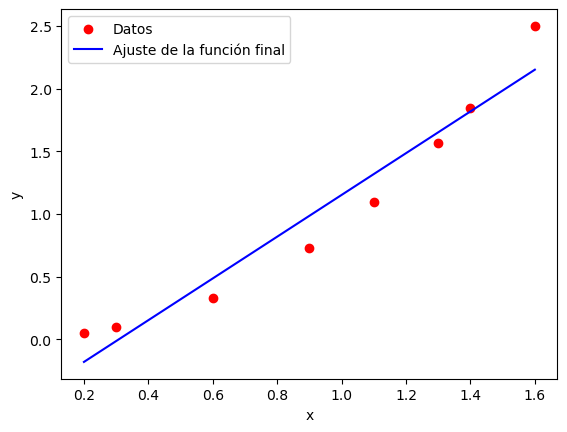
\includegraphics{Tarea8_MN_files/figure-pdf/cell-10-output-2.png}

\subsubsection{Literal b)}\label{literal-b-1}

Construya el polinomio por mínimos cuadrados de grado 2 y calcule el
error.

\begin{Shaded}
\begin{Highlighting}[]

\KeywordTok{def}\NormalTok{ func(x, a, b, c):}
    \ControlFlowTok{return}\NormalTok{ a}\OperatorTok{*}\NormalTok{x}\OperatorTok{**}\DecValTok{2} \OperatorTok{+}\NormalTok{ b}\OperatorTok{*}\NormalTok{x }\OperatorTok{+}\NormalTok{ c}

\CommentTok{\# Minimizando el error}
\NormalTok{popt, pcov }\OperatorTok{=}\NormalTok{ curve\_fit(func, x\_ej2, y\_ej2)}
\NormalTok{a, b, c }\OperatorTok{=}\NormalTok{ popt}

\CommentTok{\# Imprimiendo la función resultante y el error}
\NormalTok{x\_sym }\OperatorTok{=}\NormalTok{ sym.symbols(}\StringTok{"x"}\NormalTok{)}
\NormalTok{func\_sym }\OperatorTok{=} \BuiltInTok{round}\NormalTok{(a, }\DecValTok{2}\NormalTok{)}\OperatorTok{*}\NormalTok{x\_sym}\OperatorTok{**}\DecValTok{2} \OperatorTok{+} \BuiltInTok{round}\NormalTok{(b, }\DecValTok{2}\NormalTok{)}\OperatorTok{*}\NormalTok{x\_sym }\OperatorTok{+} \BuiltInTok{round}\NormalTok{(c, }\DecValTok{2}\NormalTok{)}
\BuiltInTok{print}\NormalTok{(}\SpecialStringTok{f"La función resultante es: }\SpecialCharTok{\{}\NormalTok{func\_sym}\SpecialCharTok{\}}\SpecialStringTok{"}\NormalTok{)}

\NormalTok{r\_error }\OperatorTok{=}\NormalTok{ calculate\_error(}\KeywordTok{lambda}\NormalTok{ x: a}\OperatorTok{*}\NormalTok{x}\OperatorTok{**}\DecValTok{2} \OperatorTok{+}\NormalTok{ b}\OperatorTok{*}\NormalTok{x }\OperatorTok{+}\NormalTok{ c, x\_ej2, y\_ej2)}
\BuiltInTok{print}\NormalTok{(}\SpecialStringTok{f"El error relativo en todos los puntos promedio es: }\SpecialCharTok{\{}\NormalTok{r\_error}\SpecialCharTok{\}}\SpecialStringTok{"}\NormalTok{)}

\CommentTok{\# Graficando}
\NormalTok{leasts\_squares\_graphic(}\KeywordTok{lambda}\NormalTok{ x: a}\OperatorTok{*}\NormalTok{x}\OperatorTok{**}\DecValTok{2} \OperatorTok{+}\NormalTok{ b}\OperatorTok{*}\NormalTok{x }\OperatorTok{+}\NormalTok{ c, x\_ej2, y\_ej2)}
\end{Highlighting}
\end{Shaded}

\begin{verbatim}
La función resultante es: 1.13*x**2 - 0.31*x + 0.09
El error relativo en todos los puntos promedio es: 0.8305132456280757
\end{verbatim}

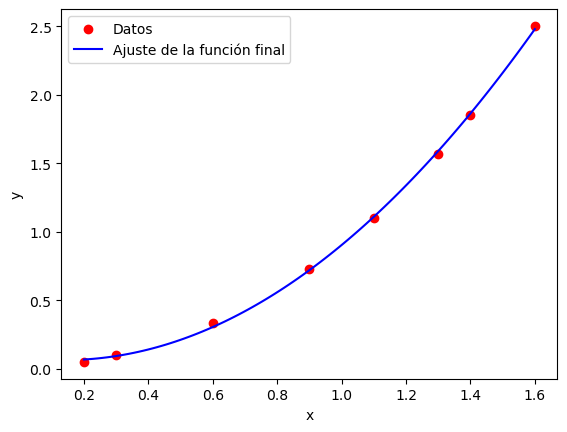
\includegraphics{Tarea8_MN_files/figure-pdf/cell-11-output-2.png}

\subsubsection{Literal c)}\label{literal-c-1}

Construya el polinomio por mínimos cuadrados de grado 3 y calcule el
error.

\begin{Shaded}
\begin{Highlighting}[]

\KeywordTok{def}\NormalTok{ func(x, a, b, c, d):}
    \ControlFlowTok{return}\NormalTok{ a}\OperatorTok{*}\NormalTok{x}\OperatorTok{**}\DecValTok{3} \OperatorTok{+}\NormalTok{ b}\OperatorTok{*}\NormalTok{x}\OperatorTok{**}\DecValTok{2} \OperatorTok{+}\NormalTok{ c}\OperatorTok{*}\NormalTok{x }\OperatorTok{+}\NormalTok{ d}

\CommentTok{\# Minimizando el error}
\NormalTok{popt, pcov }\OperatorTok{=}\NormalTok{ curve\_fit(func, x\_ej2, y\_ej2)}
\NormalTok{a, b, c, d }\OperatorTok{=}\NormalTok{ popt}

\CommentTok{\# Imprimiendo la función resultante y el error}
\NormalTok{x\_sym }\OperatorTok{=}\NormalTok{ sym.symbols(}\StringTok{"x"}\NormalTok{)}
\NormalTok{func\_sym }\OperatorTok{=} \BuiltInTok{round}\NormalTok{(a, }\DecValTok{2}\NormalTok{)}\OperatorTok{*}\NormalTok{x\_sym}\OperatorTok{**}\DecValTok{3} \OperatorTok{+} \BuiltInTok{round}\NormalTok{(b, }\DecValTok{2}\NormalTok{)}\OperatorTok{*}\NormalTok{x\_sym}\OperatorTok{**}\DecValTok{2} \OperatorTok{+} \BuiltInTok{round}\NormalTok{(c, }\DecValTok{2}\NormalTok{)}\OperatorTok{*}\NormalTok{x\_sym }\OperatorTok{+} \BuiltInTok{round}\NormalTok{(d, }\DecValTok{2}\NormalTok{)}
\BuiltInTok{print}\NormalTok{(}\SpecialStringTok{f"La función resultante es: }\SpecialCharTok{\{}\NormalTok{func\_sym}\SpecialCharTok{\}}\SpecialStringTok{"}\NormalTok{)}

\NormalTok{r\_error }\OperatorTok{=}\NormalTok{ calculate\_error(}\KeywordTok{lambda}\NormalTok{ x: a}\OperatorTok{*}\NormalTok{x}\OperatorTok{**}\DecValTok{3} \OperatorTok{+}\NormalTok{ b}\OperatorTok{*}\NormalTok{x}\OperatorTok{**}\DecValTok{2} \OperatorTok{+}\NormalTok{ c}\OperatorTok{*}\NormalTok{x }\OperatorTok{+}\NormalTok{ d, x\_ej2, y\_ej2)}
\BuiltInTok{print}\NormalTok{(}\SpecialStringTok{f"El error relativo en todos los puntos promedio es: }\SpecialCharTok{\{}\NormalTok{r\_error}\SpecialCharTok{\}}\SpecialStringTok{"}\NormalTok{)}

\CommentTok{\# Graficando}
\NormalTok{leasts\_squares\_graphic(}\KeywordTok{lambda}\NormalTok{ x: a}\OperatorTok{*}\NormalTok{x}\OperatorTok{**}\DecValTok{3} \OperatorTok{+}\NormalTok{ b}\OperatorTok{*}\NormalTok{x}\OperatorTok{**}\DecValTok{2} \OperatorTok{+}\NormalTok{ c}\OperatorTok{*}\NormalTok{x }\OperatorTok{+}\NormalTok{ d, x\_ej2, y\_ej2)}
\end{Highlighting}
\end{Shaded}

\begin{verbatim}
La función resultante es: 0.27*x**3 + 0.4*x**2 + 0.25*x - 0.02
El error relativo en todos los puntos promedio es: 0.8549642457850933
\end{verbatim}

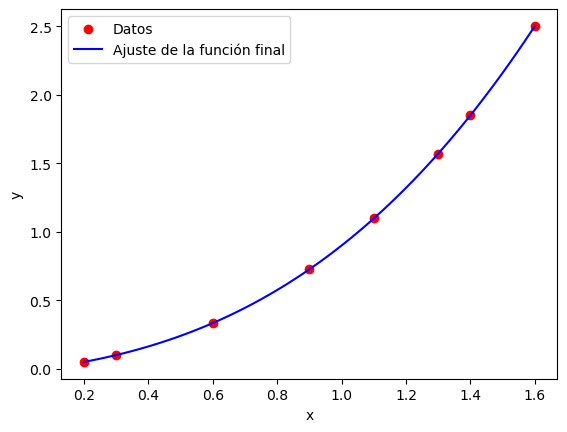
\includegraphics{Tarea8_MN_files/figure-pdf/cell-12-output-2.png}

\subsubsection{Literal d)}\label{literal-d-1}

Construya el polinomio por mínimos cuadrados de la forma \(be^{ax}\) y
calcule el error.

\begin{Shaded}
\begin{Highlighting}[]

\KeywordTok{def}\NormalTok{ func(x, a, b):}
    \ControlFlowTok{return}\NormalTok{ b}\OperatorTok{*}\NormalTok{np.exp(a}\OperatorTok{*}\NormalTok{x)}

\CommentTok{\# Minimizando el error}
\NormalTok{popt, pcov }\OperatorTok{=}\NormalTok{ curve\_fit(func, x\_ej2, y\_ej2)}
\NormalTok{a, b }\OperatorTok{=}\NormalTok{ popt}

\CommentTok{\# Imprimiendo la función resultante y el error}
\NormalTok{x\_sym }\OperatorTok{=}\NormalTok{ sym.symbols(}\StringTok{"x"}\NormalTok{)}
\NormalTok{func\_sym }\OperatorTok{=} \BuiltInTok{round}\NormalTok{(b, }\DecValTok{2}\NormalTok{)}\OperatorTok{*}\NormalTok{sym.exp(}\BuiltInTok{round}\NormalTok{(a, }\DecValTok{2}\NormalTok{)}\OperatorTok{*}\NormalTok{x\_sym)}
\BuiltInTok{print}\NormalTok{(}\SpecialStringTok{f"La función resultante es: }\SpecialCharTok{\{}\NormalTok{func\_sym}\SpecialCharTok{\}}\SpecialStringTok{"}\NormalTok{)}

\NormalTok{r\_error }\OperatorTok{=}\NormalTok{ calculate\_error(}\KeywordTok{lambda}\NormalTok{ x: b}\OperatorTok{*}\NormalTok{np.exp(a}\OperatorTok{*}\NormalTok{x), x\_ej2, y\_ej2)}
\BuiltInTok{print}\NormalTok{(}\SpecialStringTok{f"El error relativo en todos los puntos promedio es: }\SpecialCharTok{\{}\NormalTok{r\_error}\SpecialCharTok{\}}\SpecialStringTok{"}\NormalTok{)}

\CommentTok{\# Graficando}
\NormalTok{leasts\_squares\_graphic(}\KeywordTok{lambda}\NormalTok{ x: b}\OperatorTok{*}\NormalTok{np.exp(a}\OperatorTok{*}\NormalTok{x), x\_ej2, y\_ej2)}
\end{Highlighting}
\end{Shaded}

\begin{verbatim}
La función resultante es: 0.13*exp(1.86*x)
El error relativo en todos los puntos promedio es: 0.3122099285167875
\end{verbatim}

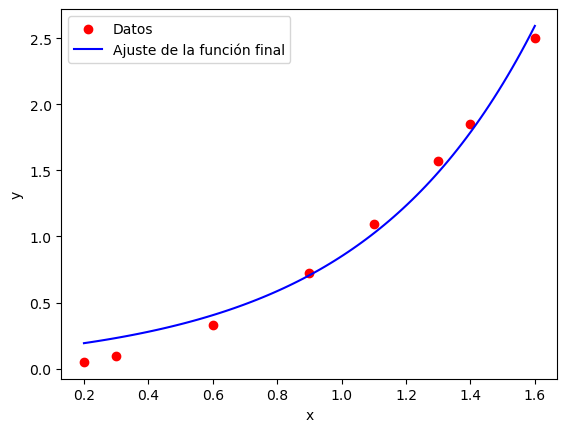
\includegraphics{Tarea8_MN_files/figure-pdf/cell-13-output-2.png}

\subsubsection{Literal e)}\label{literal-e-1}

Construya el polinomio por mínimos cuadrados de la forma \(bx^a\) y
calcule el error.

\begin{Shaded}
\begin{Highlighting}[]

\KeywordTok{def}\NormalTok{ func(x, a, b):}
    \ControlFlowTok{return}\NormalTok{ b}\OperatorTok{*}\NormalTok{x}\OperatorTok{**}\NormalTok{a}

\CommentTok{\# Minimizando el error}
\NormalTok{popt, pcov }\OperatorTok{=}\NormalTok{ curve\_fit(func, x\_ej2, y\_ej2)}
\NormalTok{a, b }\OperatorTok{=}\NormalTok{ popt}

\CommentTok{\# Imprimiendo la función resultante y el error}
\NormalTok{x\_sym }\OperatorTok{=}\NormalTok{ sym.symbols(}\StringTok{"x"}\NormalTok{)}
\NormalTok{func\_sym }\OperatorTok{=} \BuiltInTok{round}\NormalTok{(b, }\DecValTok{2}\NormalTok{)}\OperatorTok{*}\NormalTok{x\_sym}\OperatorTok{**}\BuiltInTok{round}\NormalTok{(a, }\DecValTok{2}\NormalTok{)}
\BuiltInTok{print}\NormalTok{(}\SpecialStringTok{f"La función resultante es: }\SpecialCharTok{\{}\NormalTok{func\_sym}\SpecialCharTok{\}}\SpecialStringTok{"}\NormalTok{)}

\NormalTok{r\_error }\OperatorTok{=}\NormalTok{ calculate\_error(}\KeywordTok{lambda}\NormalTok{ x: b}\OperatorTok{*}\NormalTok{x}\OperatorTok{**}\NormalTok{a, x\_ej2, y\_ej2)}
\BuiltInTok{print}\NormalTok{(}\SpecialStringTok{f"El error relativo en todos los puntos promedio es: }\SpecialCharTok{\{}\NormalTok{r\_error}\SpecialCharTok{\}}\SpecialStringTok{"}\NormalTok{)}

\CommentTok{\# Graficando}
\NormalTok{leasts\_squares\_graphic(}\KeywordTok{lambda}\NormalTok{ x: b}\OperatorTok{*}\NormalTok{x}\OperatorTok{**}\NormalTok{a, x\_ej2, y\_ej2)}
\end{Highlighting}
\end{Shaded}

\begin{verbatim}
La función resultante es: 0.91*x**2.14
El error relativo en todos los puntos promedio es: 0.9595557974073141
\end{verbatim}

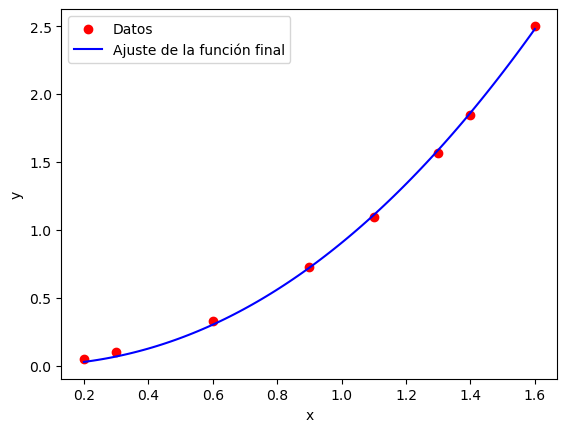
\includegraphics{Tarea8_MN_files/figure-pdf/cell-14-output-2.png}

\subsection{Ejercicio 3}\label{ejercicio-3}

La siguiente tabla muestra los promedios de puntos del colegio de 20
especialistas en matemáticas y ciencias computacionales, junto con las
calificaciones que recibieron estos estudiantes en la parte de
matemáticas de la prueba ACT (Programa de Pruebas de Colegios
Americanos) mientras estaban en secundaria. Grafique estos datos y
encuentre la ecuación de la recta por mínimos cuadrados.

\begin{Shaded}
\begin{Highlighting}[]

\NormalTok{punt\_ATC }\OperatorTok{=}\NormalTok{ [}\DecValTok{28}\NormalTok{, }\DecValTok{25}\NormalTok{, }\DecValTok{28}\NormalTok{, }\DecValTok{27}\NormalTok{, }\DecValTok{28}\NormalTok{, }\DecValTok{33}\NormalTok{, }\DecValTok{28}\NormalTok{, }\DecValTok{29}\NormalTok{, }\DecValTok{23}\NormalTok{, }\DecValTok{27}\NormalTok{,}
            \DecValTok{29}\NormalTok{, }\DecValTok{28}\NormalTok{, }\DecValTok{27}\NormalTok{, }\DecValTok{29}\NormalTok{, }\DecValTok{21}\NormalTok{, }\DecValTok{28}\NormalTok{, }\DecValTok{28}\NormalTok{, }\DecValTok{26}\NormalTok{, }\DecValTok{30}\NormalTok{, }\DecValTok{24}\NormalTok{]}
\NormalTok{prom\_puntos }\OperatorTok{=}\NormalTok{ [}\FloatTok{3.84}\NormalTok{, }\FloatTok{3.21}\NormalTok{, }\FloatTok{3.23}\NormalTok{, }\FloatTok{3.63}\NormalTok{, }\FloatTok{3.75}\NormalTok{, }\FloatTok{3.20}\NormalTok{, }\FloatTok{3.41}\NormalTok{, }\FloatTok{3.38}\NormalTok{, }\FloatTok{3.53}\NormalTok{, }\FloatTok{2.03}\NormalTok{, }
               \FloatTok{3.75}\NormalTok{, }\FloatTok{3.65}\NormalTok{, }\FloatTok{3.87}\NormalTok{, }\FloatTok{3.75}\NormalTok{, }\FloatTok{1.66}\NormalTok{, }\FloatTok{3.12}\NormalTok{, }\FloatTok{2.96}\NormalTok{, }\FloatTok{2.92}\NormalTok{, }\FloatTok{3.1}\NormalTok{, }\FloatTok{2.81}\NormalTok{]}
\end{Highlighting}
\end{Shaded}

\subsection{Puntos de los datos correspondientes al ejercicio
3}\label{puntos-de-los-datos-correspondientes-al-ejercicio-3}

\begin{Shaded}
\begin{Highlighting}[]

\NormalTok{plt.scatter(punt\_ATC, prom\_puntos, label}\OperatorTok{=}\StringTok{\textquotesingle{}Datos\textquotesingle{}}\NormalTok{, color}\OperatorTok{=}\StringTok{\textquotesingle{}red\textquotesingle{}}\NormalTok{)}
\NormalTok{plt.xlabel(}\StringTok{"x"}\NormalTok{)}
\NormalTok{plt.ylabel(}\StringTok{"y"}\NormalTok{)}
\NormalTok{plt.legend()}
\NormalTok{plt.show()}
\end{Highlighting}
\end{Shaded}

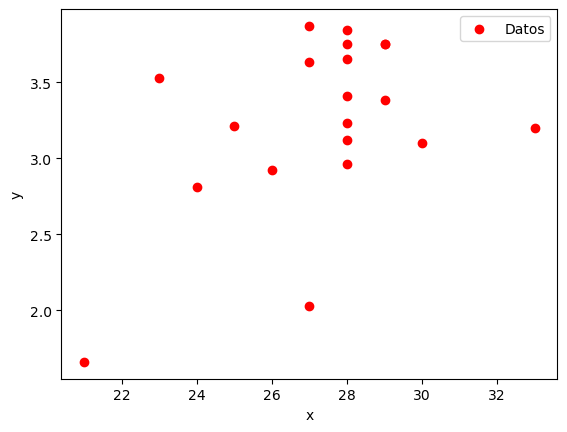
\includegraphics{Tarea8_MN_files/figure-pdf/cell-16-output-1.png}

\begin{Shaded}
\begin{Highlighting}[]

\KeywordTok{def}\NormalTok{ func(x, a, b):}
    \ControlFlowTok{return}\NormalTok{ a}\OperatorTok{*}\NormalTok{x }\OperatorTok{+}\NormalTok{ b}

\CommentTok{\# Minimizando el error}
\NormalTok{popt, pcov }\OperatorTok{=}\NormalTok{ curve\_fit(func, punt\_ATC, prom\_puntos)}
\NormalTok{a, b }\OperatorTok{=}\NormalTok{ popt}

\CommentTok{\# Imprimiendo la función resultante}
\NormalTok{x\_sym }\OperatorTok{=}\NormalTok{ sym.symbols(}\StringTok{"x"}\NormalTok{)}
\NormalTok{func\_sym }\OperatorTok{=} \BuiltInTok{round}\NormalTok{(a, }\DecValTok{2}\NormalTok{)}\OperatorTok{*}\NormalTok{x\_sym }\OperatorTok{+} \BuiltInTok{round}\NormalTok{(b, }\DecValTok{2}\NormalTok{)}
\BuiltInTok{print}\NormalTok{(}\SpecialStringTok{f"La función resultante es: }\SpecialCharTok{\{}\NormalTok{func\_sym}\SpecialCharTok{\}}\SpecialStringTok{"}\NormalTok{)}

\CommentTok{\# Graficando}
\NormalTok{leasts\_squares\_graphic(}\KeywordTok{lambda}\NormalTok{ x: a}\OperatorTok{*}\NormalTok{x }\OperatorTok{+}\NormalTok{ b, punt\_ATC, prom\_puntos)}
\end{Highlighting}
\end{Shaded}

\begin{verbatim}
La función resultante es: 0.1*x + 0.49
\end{verbatim}

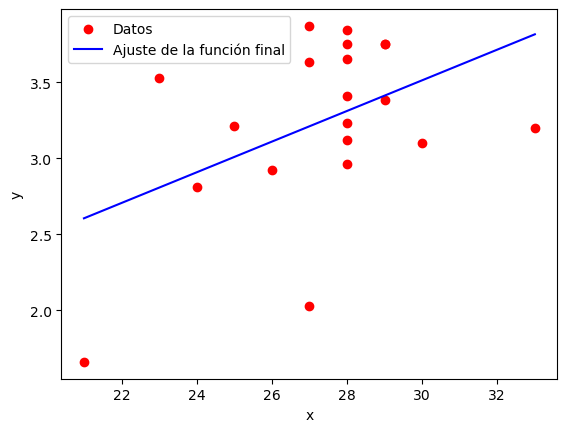
\includegraphics{Tarea8_MN_files/figure-pdf/cell-17-output-2.png}

Los puntos en el gráfico de dispersión no siguen una tendencia clara y
están alejados de la línea de regresión. \#\# Ejercicio 4

El siguiente conjunto de datos, presentado al Subcomité Antimonopolio
del Senado, muestra las características comparativas de supervivencia
durante un choque de automóviles de diferentes clases. Encuentre la
recta por mínimos cuadrados que aproxima estos datos (la tabla muest el
porcentaje de vehículos que participaron en un accidente en los que la
lesión más grave fue fatal o seria).ra

\begin{Shaded}
\begin{Highlighting}[]
\NormalTok{peso\_prom }\OperatorTok{=}\NormalTok{ [}\DecValTok{4800}\NormalTok{, }\DecValTok{3700}\NormalTok{, }\DecValTok{3400}\NormalTok{, }\DecValTok{2800}\NormalTok{, }\DecValTok{1900}\NormalTok{]}
\NormalTok{porc\_pres }\OperatorTok{=}\NormalTok{ [}\FloatTok{3.1}\NormalTok{, }\DecValTok{4}\NormalTok{, }\FloatTok{5.2}\NormalTok{, }\FloatTok{6.4}\NormalTok{, }\FloatTok{9.6}\NormalTok{]}
\end{Highlighting}
\end{Shaded}

Primero graficamos los puntos en el plano cartesiano:

\begin{Shaded}
\begin{Highlighting}[]

\NormalTok{plt.scatter(peso\_prom, porc\_pres, label}\OperatorTok{=}\StringTok{\textquotesingle{}Datos\textquotesingle{}}\NormalTok{, color}\OperatorTok{=}\StringTok{\textquotesingle{}red\textquotesingle{}}\NormalTok{)}
\NormalTok{plt.xlabel(}\StringTok{"x"}\NormalTok{)}
\NormalTok{plt.ylabel(}\StringTok{"y"}\NormalTok{)}
\NormalTok{plt.legend()}
\NormalTok{plt.show()}
\end{Highlighting}
\end{Shaded}

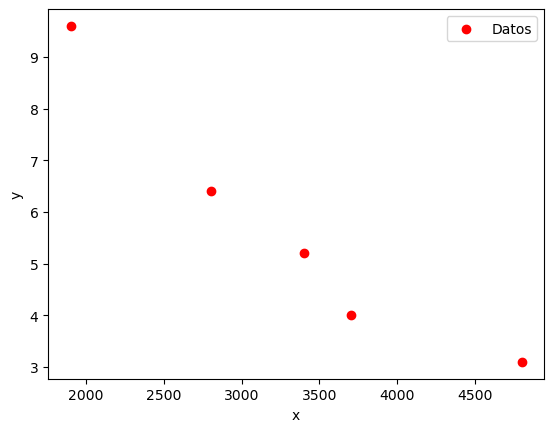
\includegraphics{Tarea8_MN_files/figure-pdf/cell-19-output-1.png}

Tal parece que nos conviene más una función cuadrática, ya que se ajusta
a la mitad de una. Entonces llamamos nuestro algoritmo:

\begin{Shaded}
\begin{Highlighting}[]

\KeywordTok{def}\NormalTok{ func(x, a, b, c):}
    \ControlFlowTok{return}\NormalTok{ a}\OperatorTok{*}\NormalTok{x}\OperatorTok{**}\DecValTok{2} \OperatorTok{+}\NormalTok{ b}\OperatorTok{*}\NormalTok{x }\OperatorTok{+}\NormalTok{ c}

\CommentTok{\# Minimizando el error}
\NormalTok{popt, pcov }\OperatorTok{=}\NormalTok{ curve\_fit(func, peso\_prom, porc\_pres)}
\NormalTok{a, b, c }\OperatorTok{=}\NormalTok{ popt}

\CommentTok{\# Imprimiendo la función resultante y el error}
\NormalTok{x\_sym }\OperatorTok{=}\NormalTok{ sym.symbols(}\StringTok{"x"}\NormalTok{)}
\NormalTok{func\_sym }\OperatorTok{=} \BuiltInTok{round}\NormalTok{(a, }\DecValTok{2}\NormalTok{)}\OperatorTok{*}\NormalTok{x\_sym}\OperatorTok{**}\DecValTok{2} \OperatorTok{+} \BuiltInTok{round}\NormalTok{(b, }\DecValTok{2}\NormalTok{)}\OperatorTok{*}\NormalTok{x\_sym }\OperatorTok{+} \BuiltInTok{round}\NormalTok{(c, }\DecValTok{2}\NormalTok{)}
\BuiltInTok{print}\NormalTok{(}\SpecialStringTok{f"La función resultante es: }\SpecialCharTok{\{}\NormalTok{func\_sym}\SpecialCharTok{\}}\SpecialStringTok{"}\NormalTok{)}

\CommentTok{\# Graficando}
\NormalTok{leasts\_squares\_graphic(}\KeywordTok{lambda}\NormalTok{ x: a}\OperatorTok{*}\NormalTok{x}\OperatorTok{**}\DecValTok{2} \OperatorTok{+}\NormalTok{ b}\OperatorTok{*}\NormalTok{x }\OperatorTok{+}\NormalTok{ c, peso\_prom, porc\_pres)}
\end{Highlighting}
\end{Shaded}

\begin{verbatim}
La función resultante es: 19.69 - 0.01*x
\end{verbatim}

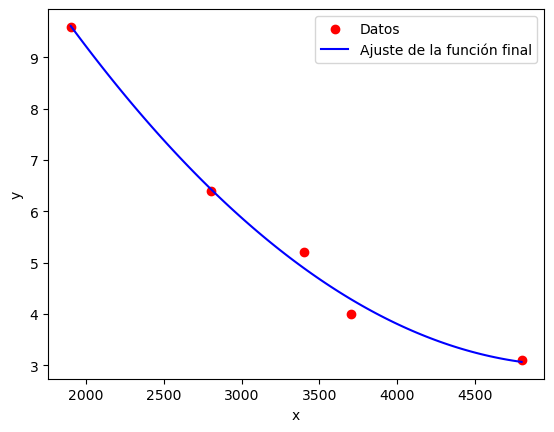
\includegraphics{Tarea8_MN_files/figure-pdf/cell-20-output-2.png}




\end{document}
